\documentclass{rapportECL}
\usepackage{amsmath}
\usepackage{fancybox}
\usepackage{lipsum}

%\usepackage{biblatex}% ojo :No se puede mezclar el comando \ bibliographystyle y el paquete biblatex. La opción style = ... se utiliza para esta función. 
% luego se pudo usar el archivo bib y referenciar

\usepackage{csquotes}
%\addbibresource{main.bib}
\usepackage{times}
\usepackage{fancyhdr,graphicx,amsmath,amssymb}
\usepackage[spanish]{babel}
\usepackage{listings}
\usepackage{xcolor}
\definecolor{codegreen}{rgb}{0,0.6,0}
\definecolor{codegray}{rgb}{0.5,0.5,0.5}
\definecolor{codepurple}{rgb}{0.58,0,0.82}
\definecolor{backcolour}{rgb}{0.95,0.95,0.92}

\lstdefinestyle{mystyle}{
    backgroundcolor=\color{backcolour},   % backcolour
    commentstyle=\color{codegreen},
    keywordstyle=\color{blue},
    numberstyle=\tiny\color{codegray},
    stringstyle=\color{codegreen},
    basicstyle=\ttfamily\footnotesize,
    breakatwhitespace=false,         
    breaklines=true,                 
    captionpos=b,                    
    keepspaces=true,                 
    numbers=left,                    
    numbersep=5pt,                  
    showspaces=false,                
    showstringspaces=false,
    showtabs=false,                  
    tabsize=2
}
\lstset{style=mystyle}\usepackage{xcolor}
\DeclareUnicodeCharacter{2212}{-}
\DeclareUnicodeCharacter{2217}{*}
\newcommand{\subsubsubsection}[1]{\paragraph{#1}\mbox{}\\}
\setcounter{secnumdepth}{4}
\setcounter{tocdepth}{4}

\title{}

\begin{document}


\titre{QuadTree}
\UE{\textbf{Escuela Profesional de Ciencia de la Computaci\'on}} %Nom de la UE
\sujet{Estructura de datos Avanzadas} %Nom du sujet

\eleves{Angel Andres  Bejar Merma\\
    \\
    \\}
\enseignant{Dra.  Evelyn Perez C.}

%----------- Initialisation -------------------

\fairemarges %Afficher les marges
\fairepagedegarde %Créer la page de garde 

\tableofcontents
\newpage

\section{Marco teórico}


Un Quadtree es una estructura de datos en la que cada nodo tiene exactamente cuatro hijos ver figura \ref{fig:arbol}.


\begin{figure}[H]%primero aqui sino arriba sino abajo
\centering
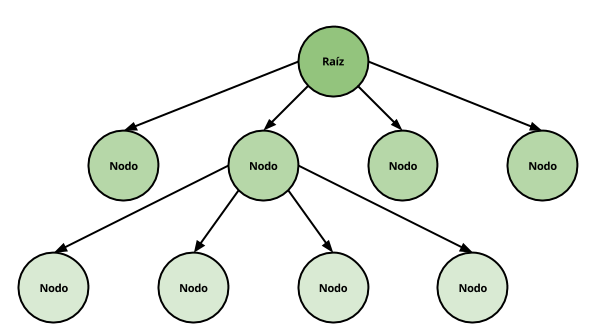
\includegraphics[width=13cm]{imagenes/tree.png}
\caption{arbol quadtree}
\label{fig:arbol}
\end{figure}



\begin{figure}[H]%primero aqui sino arriba sino abajo
\centering
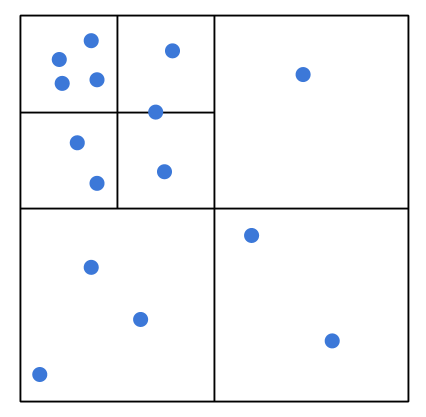
\includegraphics[width=5cm]{imagenes/cuad.png}
\caption{ representacion del  mapa }
\end{figure}


 Se construye dividiendo continuamente cada nodo hasta que cada nodo hoja solo tenga un único nodo dentro de él.Los Quadtrees se generalizan como árboles “kd / k-dimensionales” cuando tienes más de 4 divisiones en cada nodo;

Aunque generalmente se usan en dos dimensiones, los quadtrees se pueden emplear a una cantidad arbitraria de dimensiones.Lo mejor de los Quadtree es la "reducción dimensional". En lugar de operar en O ($n^2$) para una   búsqueda lineal común  en dos dimensiones, el Quadtree puede lograr un tiempo cercano a O (log n) para la mayoría de las operaciones.

\begin{figure}[H]%primero aqui sino arriba sino abajo
\centering
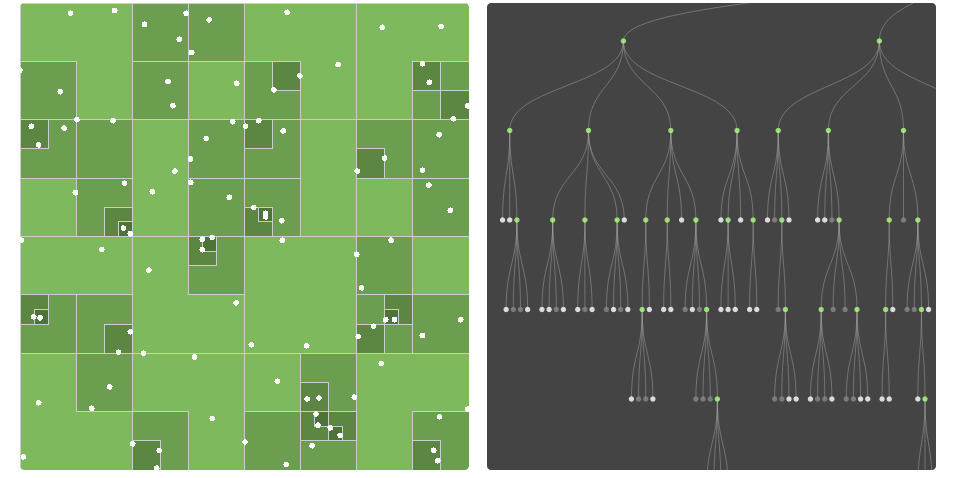
\includegraphics[width=15cm]{imagenes/quad0.png}
\caption{mejor representacion  del quadtree}
\label{fig:repre}
\end{figure}

En la figura \ref{fig:repre} cada nodo verde representa un rectángulo en un espacio.
    Cada nodo blanco representa un punto en ese mismo espacio.
    Los nodos verdes pueden tener hasta cuatro hijos , ya sean blancos o verdes. Estos hijos están contenidos dentro del rectángulo que representa el nodo verde.
    (Los nodos grises representan espacios vacíos, lugares para nodos hijos  que aún no están ocupados).
\\    
\\
Todas las formas de quadtree comparten las siguientes  características\cite{quad3} :
  
    
\begin{itemize}
    \item Descomponen el espacio en celdas adaptables.
    \item  Cada celda (o cuadrante) tiene una capacidad máxima. Cuando se alcanza la capacidad máxima, el cubo se divide
    \item    El directorio del árbol sigue la descomposición espacial del quadtree. 
\end{itemize}
\\
\\
 Algunos posibles usos de eso incluyen:

\begin{itemize}
    \item \textbf{Detección de colisiones:} Normalmente para detectar una colisión, se   compararía todos los puntos contra todos y si  fueran  1000 puntos y ninguno de ellos fuera una colisión se tendría que hacerse 1000*1000 comprobaciones lo que es un desperdicio de tiempo y rendimiento.
 
   Así que aquí entra en acción el  Quadtree, cuando tenga que buscar , dividirá el mapa en cuadrantes y así hará una comprobación por cuadrante ahorrando tiempo y mejorando el costo. Luego, descubrirá en qué cuadrante dentro de ese cuadrante se encuentra y así recursivamente hasta llegar a la colisión.

    En ese sentido solo se tendrá que hacer esto como máximo siete veces para un espacio de 100x100 (asumiendo que los puntos solo pueden tener valores enteros), incluso si hay 1000 puntos en él. Para un espacio de 1,000,000x1,000,000, es un máximo de 20 veces.
        \item\textbf{ Encontrar al vecino más cercano:} Se tiene un mapa de puntos ,en lugar de preguntarse si alguno de ellos coincide con un punto dado, podrías pensar se cuál es el punto más cercano que tienes a un punto arbitrario entre tus puntos.


                    
\end{itemize}


\section{Metodologia}

  
Para una mejor comprensión del funcionamiento del quadtree puede visitar \cite{pagina}.
En la metodología :     

 \begin{itemize}
     \item Se probo empleo Python en una plataforma linux y creando un entorno virtual \cite{video}
     \item  La computadora  que utilizo fue una intel i5 de quinta generación  con 2 cores ,8 gb  de memoria ram.
     \item  Se creó dos archivos el primero para probar,  test.py donde se importan las funciones definidas en  las clases   del segundo archivo quadtree.py.
     
     \item \textit{La estructura de código es el siguiente :}
Se implementó   tres principales clases: punto ,rectángulo y Quadtree \cite{quadtreepage}.
En esta última se definieron las funciones más importantes  \textit{insertar} y \textit{consultar rango}.
Para la primera parte  se crearon puntos de forma aleatoria,


     
 \end{itemize}
 
Para la \textbf{inserción}, primero se  verifica si el nodo dado está dentro de los límites del quadtree actual . Si no es así, dejamos de insertar inmediatamente y si sobre pasa la capacidad llamamos a la función divide para dividir la celda y empezar de nuevo el proceso. Entonces si está dentro de los límites, seleccionamos el hijo apropiado para contener este nodo en función de su ubicación.
Esta función es O (Log N) donde N es el tamaño de la distancia.
 









\section{Resultados}



\subsection{probando con 50 elementos }

Estableciendo N=50 .






   

   .

   



\begin{figure}[H]
  \centering
  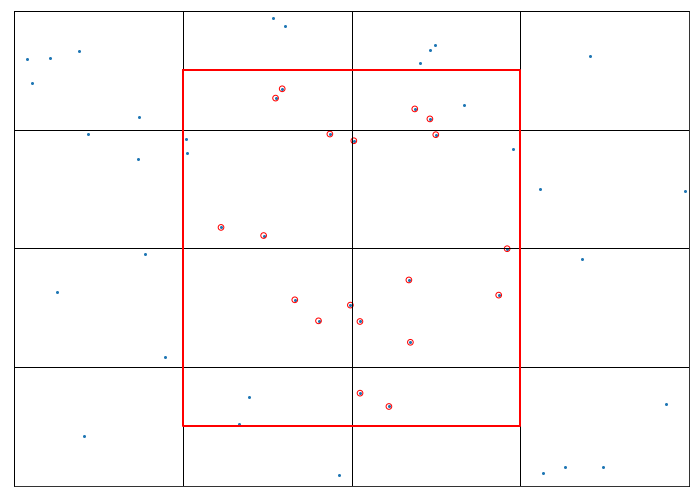
\includegraphics[width=0.8\textwidth]{imagenes/search-quadtree.png}
 % \label{fig:act-1}
\end{figure}


\begin{figure}[H]
  \centering
  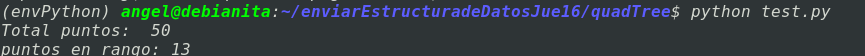
\includegraphics[width=1\textwidth]{imagenes/rango.png}
 % \label{fig:act-1}
\end{figure}

En la figura  el rango osea la cantidad de puntos  dentro del cuadrado rojo son 13 \cite{repo}.

\section{discusión}



 Quadtree no trabaja bien  cuando debe almacenar gran cantidad de diferentes píxeles existentes en una imagen con muchos colores, dado que podría tomar un tamaño excesivamente grande.
    También por ser una estructura de datos de memoria principal, al querer representar imágenes muy grandes, muchas veces el Quadtree no puede ser almacenado en dicha memoria. En esos caso, es mejor usar  estructuras alternativas por ejemplo, un B+ tree, para compensar esa limitación.


\section{conclusión}

Los Quadtrees son una forma de dividir el espacio para que sea fácil de intersecar y buscar.
La detección de colisiones puede ser una operación costosa y puede ralentizar el rendimiento  . Los Quadtrees son una forma en que puede ayudar a acelerar la detección de colisiones y mantener por ejemplo un juego funcionando a la máxima velocidad.




\bibliographystyle{plain}

\bibliography{main.bib}

%\printbibliography[heading=bibintoc]

\end{document}